\documentclass[10pt,aspectratio=169]{beamer}
\usepackage[utf8]{inputenc}
\usepackage[T1]{fontenc}
\usepackage[french]{babel}
\usepackage{amssymb}
\usepackage{booktabs}
\usepackage{graphicx}
\usepackage{inconsolata}
\usepackage{listings}
\usepackage{microtype}
\usepackage{tikz}
\usepackage{xcolor}
\usetikzlibrary{arrows.meta,positioning}

\definecolor{ink}{HTML}{202124}
\definecolor{muted}{HTML}{5F6368}
\definecolor{line}{HTML}{DADCE0}
\definecolor{paper}{HTML}{F8F9FA}
\definecolor{accent}{HTML}{8A1538}
\definecolor{green}{HTML}{0B6B57}
\definecolor{blue}{HTML}{245B8E}
\definecolor{amber}{HTML}{9A5B00}

\setbeamercolor{normal text}{fg=ink,bg=white}
\setbeamercolor{structure}{fg=accent}
\setbeamercolor{frametitle}{fg=ink,bg=white}
\setbeamercolor{title}{fg=ink}
\setbeamercolor{subtitle}{fg=muted}
\setbeamercolor{block title}{fg=white,bg=accent}
\setbeamercolor{block body}{fg=ink,bg=paper}
\setbeamercolor{alerted text}{fg=accent}

\setbeamertemplate{navigation symbols}{}
\setbeamertemplate{itemize item}{\color{accent}\small$\blacktriangleright$}
\setbeamertemplate{itemize subitem}{\color{green}\scriptsize$\bullet$}
\setbeamertemplate{frametitle}{
  \vspace{0.15cm}
  \insertframetitle\par
  \vspace{0.1cm}
  {\color{line}\rule{\linewidth}{0.45pt}}
}
\setbeamertemplate{footline}{
  \leavevmode%
  \hbox{%
    \begin{beamercolorbox}[wd=.76\paperwidth,ht=2.5ex,dp=1ex,leftskip=0.35cm]{author in head/foot}%
      Python pour économistes -- L2 Économie
    \end{beamercolorbox}%
    \begin{beamercolorbox}[wd=.24\paperwidth,ht=2.5ex,dp=1ex,rightskip=0.35cm plus1fil]{date in head/foot}%
      \hfill\insertframenumber/\inserttotalframenumber
    \end{beamercolorbox}%
  }%
}

\setbeamersize{text margin left=0.65cm,text margin right=0.65cm}


\lstdefinelanguage{terminal}{
  morekeywords={ls,cd,pwd,mkdir,python,python3,code,dir,type,echo},
  sensitive=true
}

\lstset{
  basicstyle=\ttfamily\small,
  backgroundcolor=\color{paper},
  frame=single,
  framerule=0.35pt,
  rulecolor=\color{line},
  keywordstyle=\color{accent}\bfseries,
  commentstyle=\color{muted},
  stringstyle=\color{green},
  showstringspaces=false,
  breaklines=true,
  columns=fullflexible,
  keepspaces=true,
  upquote=true,
  language=Python,
  literate=
   {à}{{\`a}}1 {â}{{\^a}}1 {ä}{{\"a}}1
   {ç}{{\c c}}1
   {é}{{\'e}}1 {è}{{\`e}}1 {ê}{{\^e}}1 {ë}{{\"e}}1
   {î}{{\^\i}}1 {ï}{{\"\i}}1
   {ô}{{\^o}}1 {ö}{{\"o}}1
   {ù}{{\`u}}1 {û}{{\^u}}1 {ü}{{\"u}}1
   {À}{{\`A}}1 {Â}{{\^A}}1 {Ä}{{\"A}}1
   {Ç}{{\c C}}1
   {É}{{\'E}}1 {È}{{\`E}}1 {Ê}{{\^E}}1 {Ë}{{\"E}}1
   {Î}{{\^I}}1 {Ï}{{\"I}}1
   {Ô}{{\^O}}1 {Ö}{{\"O}}1
   {Ù}{{\`U}}1 {Û}{{\^U}}1 {Ü}{{\"U}}1
   {œ}{{\oe}}1 {Œ}{{\OE}}1
   {–}{{--}}1 {—}{{---}}1
}

\newcommand{\code}[1]{\texttt{#1}}
\newcommand{\lesson}[1]{\textbf{\textcolor{accent}{#1}}}
\newcommand{\muted}[1]{\textcolor{muted}{#1}}


\title{Cours 1 -- Premiers pas avec Python}
\subtitle{Du 0/1 au script : comprendre ce que Python permet de faire}
\author{Etienne Dagorn}
\institute{Université de Lille -- L2 Économie}
\date{2026--2027}

\begin{document}

\begin{frame}
  \titlepage
\end{frame}

\begin{frame}{Pourquoi ce cours existe}
\begin{block}{But du cours}
Vous rendre capables de produire un petit script fiable, lisible et exécutable dans les TD.
\end{block}
\begin{itemize}
  \item Pas besoin de tout connaître pour commencer.
  \item Il faut surtout savoir organiser son dossier, exécuter le bon fichier et lire les erreurs simples.
  \item Le TD1 transforme ces idées en gestes obligatoires.
\end{itemize}
\end{frame}

\begin{frame}{Le parcours du semestre}
\begin{tabular}{@{}lll@{}}
\toprule
Séance & Support & Compétence principale \\
\midrule
Cours 1 & CM & Script, variables, erreurs \\
TD1 & Livret & Installation et premiers scripts \\
TD2 & Livret & Listes, dictionnaires, fonctions \\
Cours 2 & CM & Données, tableaux, description \\
TD3 & Livret & Statistiques et graphiques \\
TD4 & Livret & Graphiques et simulation simple \\
TD5 & Livret & CSV, pandas et mini-projet descriptif \\
\bottomrule
\end{tabular}
\end{frame}

\begin{frame}{La règle de travail}
\begin{block}{Un bon script de débutant}
Un bon script ne fait pas beaucoup de choses. Il fait peu de choses, mais dans le bon ordre, avec des résultats que l'on peut vérifier.
\end{block}
\begin{enumerate}
  \item Créer ou charger les données.
  \item Calculer une valeur.
  \item Afficher ou exporter le résultat.
  \item Ajouter un commentaire qui explique l'interprétation.
\end{enumerate}
\end{frame}




\begin{frame}{Pourquoi une histoire avant le code ?}
\begin{block}{Le problème pédagogique}
Si l’on commence directement par \code{print()}, Python semble magique. L’objectif est de comprendre ce que Python cache, et pourquoi ce langage nous aide.
\end{block}
\begin{itemize}
  \item Les machines ne manipulent pas des “idées” : elles manipulent des représentations.
  \item Programmer consiste à transformer une méthode en instructions exécutables.
  \item L’histoire de l’informatique aide à voir que code, machine et calcul sont liés depuis longtemps.
\end{itemize}
\end{frame}

\begin{frame}{Repères historiques : calculer, coder, programmer}
\begin{tabular}{@{}p{0.17\textwidth}p{0.30\textwidth}p{0.42\textwidth}@{}}
\toprule
Période & Exemple & Idée utile pour nous \\
\midrule
1804 & Métier Jacquard & des cartes perforées commandent une machine textile \\
1843 & Ada Lovelace & un algorithme peut être écrit pour une machine générale \\
1890 & Herman Hollerith & des données administratives sont codées sur cartes perforées \\
1930--1940 & Enigma et cryptanalyse & une règle mécanique transforme un message \\
1991 & Python & un langage lisible rend la programmation plus accessible \\
\bottomrule
\end{tabular}
\vspace{0.35cm}
\begin{block}{Fil conducteur}
À chaque étape : représenter une information, appliquer une règle, produire un résultat.
\end{block}
\end{frame}

\begin{frame}{Enigma : une machine pour transformer un message}
\begin{columns}[T,totalwidth=\textwidth]
\begin{column}{0.58\textwidth}
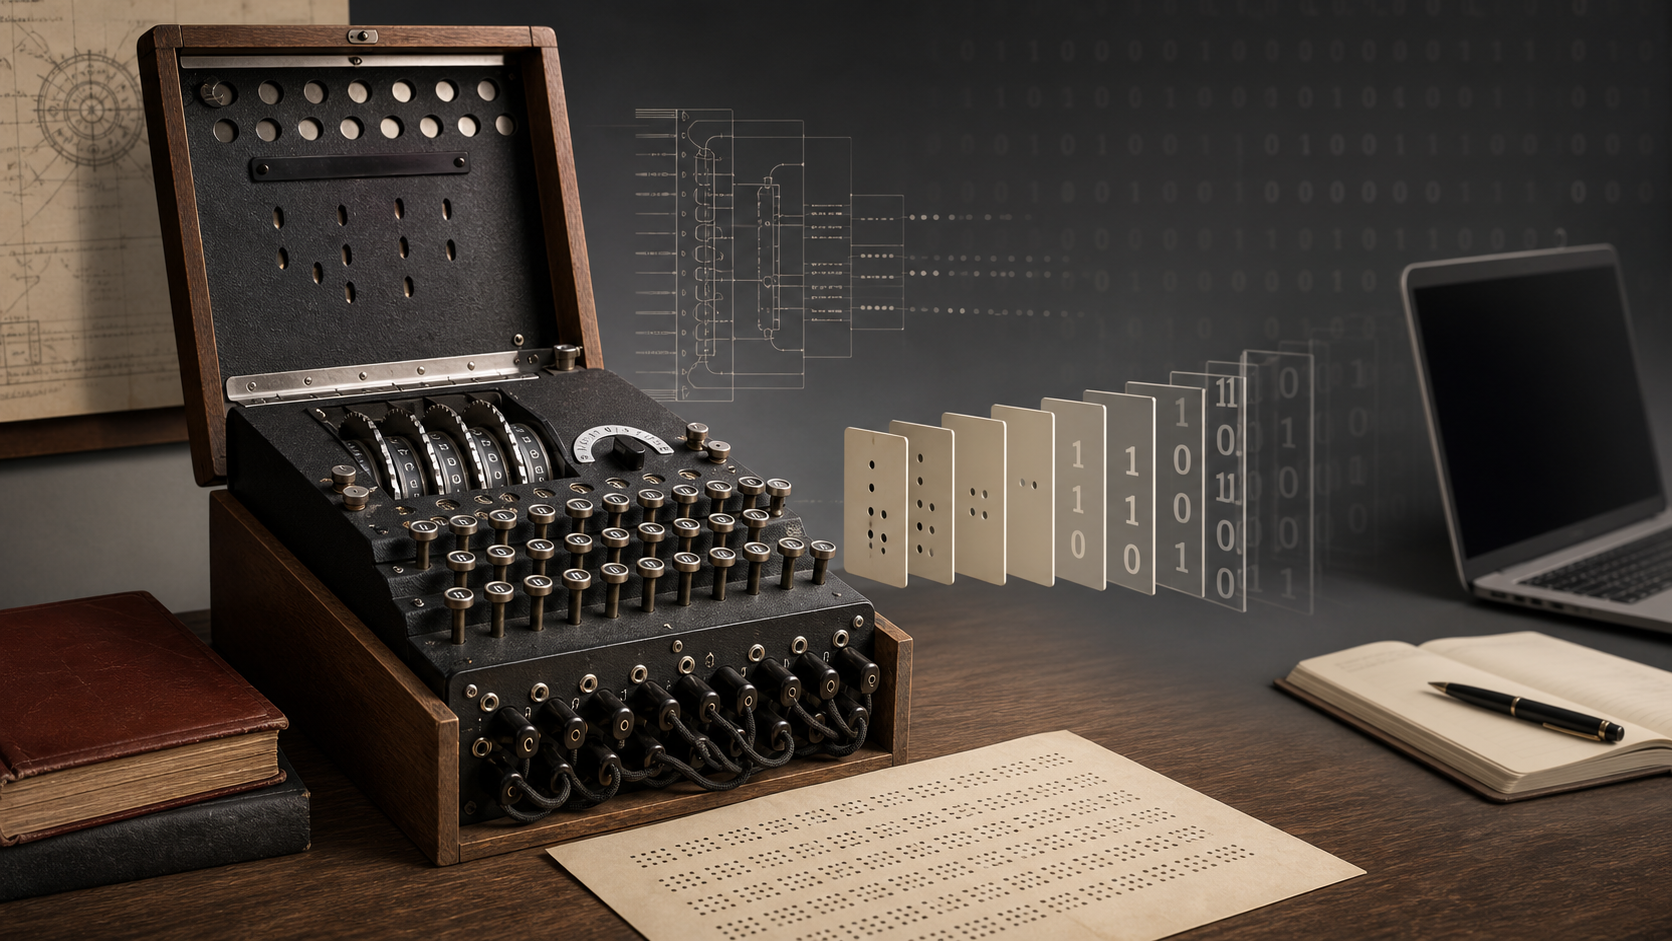
\includegraphics[width=\linewidth]{../assets/enigma_to_python.png}
\end{column}
\begin{column}{0.38\textwidth}
\begin{block}{Idée simple}
Enigma n’est pas “intelligente” : elle applique une transformation déterminée par un réglage.
\end{block}
\begin{itemize}
  \item Entrée : une lettre du message.
  \item Réglage : position des rotors.
  \item Traitement : substitutions successives.
  \item Sortie : une autre lettre.
\end{itemize}
\end{column}
\end{columns}
\end{frame}

\begin{frame}[fragile]{Enigma en pseudo-code simplifié}
Ici, on ne reproduit pas Enigma. On garde seulement la logique informatique.
\begin{lstlisting}
# Objectif : transformer un message
# Entrees : message, reglage_secret
# Pour chaque lettre du message :
#     appliquer une regle de transformation
#     ajouter la nouvelle lettre au message code
# Sortie : message code
\end{lstlisting}
\begin{block}{Lien avec Python}
Une boucle, une règle, une sortie : c’est déjà la forme de nombreux scripts de TD.
\end{block}
\end{frame}

\begin{frame}{Schéma : de l’humain à la machine}
\centering
\begin{tikzpicture}[
  node distance=0.36cm,
  box/.style={draw, rounded corners=2pt, thick, align=center, minimum width=3.0cm, minimum height=0.72cm},
  arrow/.style={-Latex, thick}
]
\node[box, fill=white, draw=accent] (human) {Question humaine\\\small calculer une moyenne};
\node[box, fill=paper, draw=blue, below=of human] (python) {Code Python\\\small \code{sum(notes) / len(notes)}};
\node[box, fill=paper, draw=green, below=of python] (interp) {Interpréteur\\\small lit et traduit};
\node[box, fill=paper, draw=amber, below=of interp] (os) {Système\\\small fichiers, mémoire, écran};
\node[box, fill=white, draw=muted, below=of os] (machine) {Machine\\\small bits, signaux, opérations};
\draw[arrow] (human) -- (python);
\draw[arrow] (python) -- (interp);
\draw[arrow] (interp) -- (os);
\draw[arrow] (os) -- (machine);
\end{tikzpicture}
\end{frame}

\begin{frame}{Schéma : une donnée change de forme}
\centering
\begin{tikzpicture}[
  node distance=0.45cm,
  box/.style={draw, rounded corners=2pt, thick, align=center, minimum width=2.35cm, minimum height=0.85cm},
  arrow/.style={-Latex, thick}
]
\node[box, fill=white, draw=accent] (letter) {Lettre\\\Large A};
\node[box, fill=paper, draw=blue, right=of letter] (number) {Nombre\\\Large 65};
\node[box, fill=paper, draw=green, right=of number] (bits) {Bits\\\Large 01000001};
\node[box, fill=white, draw=muted, right=of bits] (signal) {Signaux\\\small états physiques};
\draw[arrow] (letter) -- node[above]{codage} (number);
\draw[arrow] (number) -- node[above]{binaire} (bits);
\draw[arrow] (bits) -- node[above]{matériel} (signal);
\end{tikzpicture}
\vspace{0.45cm}
\begin{block}{Conclusion}
Python nous laisse écrire \code{"A"}, pendant que les couches inférieures gèrent les nombres, les bits et les signaux.
\end{block}
\end{frame}

\begin{frame}{Du 0/1 à Python}
\begin{block}{Idée de départ}
Un ordinateur ne comprend pas directement les phrases humaines. Au niveau matériel, tout est représenté par des états simples : présence ou absence de signal.
\end{block}
\begin{tabular}{@{}lll@{}}
\toprule
Niveau & Vocabulaire & Exemple \\
\midrule
État physique & signal & courant / pas courant \\
Bit & 0 ou 1 & \code{0}, \code{1} \\
Octet & 8 bits & \code{01000001} \\
Donnée codée & nombre ou caractère & \code{65} ou \code{"A"} \\
Programme Python & instruction lisible & \code{print("A")} \\
\bottomrule
\end{tabular}
\end{frame}

\begin{frame}{Bits, octets, conventions}
\begin{itemize}
  \item Un \textbf{bit} est une information minimale : deux possibilités, souvent notées \code{0} et \code{1}.
  \item Un \textbf{octet} regroupe 8 bits, donc il peut coder 256 valeurs différentes.
  \item La même suite de bits peut être interprétée selon une convention : nombre, lettre, couleur, son, instruction.
  \item Un fichier est essentiellement une longue suite de bits organisée selon un format.
\end{itemize}
\begin{block}{Exemple}
\code{01000001} peut être lu comme un nombre ou comme la lettre \code{A}, selon la table de codage utilisée.
\end{block}
\end{frame}

\begin{frame}{Ce que fait vraiment la machine}
\begin{block}{Processeur}
Le processeur exécute des instructions très simples : lire une valeur, écrire une valeur, additionner, comparer, sauter à une autre instruction.
\end{block}
\begin{itemize}
  \item La machine exécute très vite des opérations très petites.
  \item Les humains veulent exprimer des idées plus générales : calculer une moyenne, ouvrir un fichier, tracer un graphique.
  \item Un langage de programmation sert à faire le pont entre ces deux mondes.
\end{itemize}
\end{frame}

\begin{frame}{Les couches entre la machine et nous}
\begin{tabular}{@{}lll@{}}
\toprule
Couche & Rôle & Exemple \\
\midrule
Matériel & exécute des signaux & mémoire, processeur \\
Système d’exploitation & organise ressources et fichiers & macOS, Windows, Linux \\
Terminal & envoie des ordres textuels au système & \code{cd}, \code{pwd} \\
Interpréteur Python & lit le code Python & \code{python3} \\
Script & garde nos instructions & \code{tp1.py} \\
Bibliothèques & ajoutent des outils & \code{pandas}, \code{matplotlib} \\
\bottomrule
\end{tabular}
\vspace{0.45cm}
\begin{block}{À retenir}
Quand quelque chose bloque, il faut identifier la couche : fichier introuvable, commande introuvable, erreur Python ou erreur de logique.
\end{block}
\end{frame}

\begin{frame}{À quoi sert un langage de programmation ?}
\begin{enumerate}
  \item \textbf{Exprimer une méthode} : transformer une question en étapes.
  \item \textbf{Nommer les objets} : variables, fonctions, fichiers.
  \item \textbf{Automatiser} : refaire le même calcul sans copier-coller.
  \item \textbf{Vérifier} : relancer exactement le même script.
  \item \textbf{Partager} : permettre à quelqu’un d’autre de comprendre et reproduire.
\end{enumerate}
\begin{block}{Pour économistes}
Python sert surtout à rendre une analyse calculable, reproductible et discutable.
\end{block}
\end{frame}

\begin{frame}[fragile]{Langage : syntaxe et sens}
\begin{columns}[T,totalwidth=\textwidth]
\begin{column}{0.48\textwidth}
\begin{block}{Syntaxe}
Les règles d’écriture du langage.
\end{block}
\begin{lstlisting}
print("Bonjour")
print("Bonjour"
\end{lstlisting}
\end{column}
\begin{column}{0.48\textwidth}
\begin{block}{Sémantique}
Ce que l’instruction veut faire.
\end{block}
\begin{lstlisting}
age = 20
age = age + 1
\end{lstlisting}
\end{column}
\end{columns}
\vspace{0.35cm}
\begin{block}{Conséquence}
Une erreur de syntaxe empêche Python de lire. Une erreur de logique produit un résultat faux mais parfois sans message d’erreur.
\end{block}
\end{frame}

\begin{frame}[fragile]{Python est un langage de haut niveau}
\begin{lstlisting}
notes = [12, 15, 9, 14]
moyenne = sum(notes) / len(notes)
print(moyenne)
\end{lstlisting}
\begin{itemize}
  \item Nous écrivons des instructions lisibles par des humains.
  \item L’interpréteur Python lit ces instructions et demande au système d’exécuter les opérations nécessaires.
  \item On perd un peu de proximité avec la machine, mais on gagne énormément en lisibilité.
\end{itemize}
\end{frame}

\begin{frame}[fragile]{Exercice : replacer les niveaux}
Remettre ces éléments du plus proche de la machine au plus proche de l’utilisateur.
\begin{lstlisting}
# A. print("Bonjour")
# B. 01000001
# C. processeur
# D. script tp1.py
# E. python3
# F. systeme d exploitation
\end{lstlisting}
\pause
\begin{block}{Ordre attendu}
C puis B puis F puis E puis D puis A.
\end{block}
\end{frame}


\begin{frame}[fragile]{Exercice : coder une règle à la main}
On utilise un chiffrement très simple : remplacer chaque lettre par la suivante.
\begin{lstlisting}
# Exemple : A -> B, B -> C, C -> D
# Message : BAC
# Sortie attendue : CBD
\end{lstlisting}
\begin{enumerate}
  \item Quelle est l’entrée ?
  \item Quelle est la règle ?
  \item Quelle est la sortie ?
  \item Quelle partie deviendrait une boucle en Python ?
\end{enumerate}
\end{frame}

\begin{frame}{Informatique : six mots utiles}
\begin{tabular}{@{}lll@{}}
\toprule
Mot & Sens simple & Exemple Python \\
\midrule
Donnée & une valeur disponible & \code{22}, \code{"France"} \\
Instruction & une action demandée & \code{print(age)} \\
Algorithme & méthode en étapes & calculer une moyenne \\
Programme & algorithme écrit dans un langage & \code{tp1\_nom\_prenom.py} \\
Exécution & moment où la machine lit le programme & \code{python3 fichier.py} \\
Erreur & désaccord entre attente et réalité & \code{NameError} \\
\bottomrule
\end{tabular}
\vspace{0.35cm}
\begin{block}{Idée centrale}
Programmer, ce n’est pas “parler ordinateur” : c’est écrire une suite d’actions assez précise pour être répétée sans ambiguïté.
\end{block}
\end{frame}

\begin{frame}[fragile]{Algorithme : entrée, traitement, sortie}
\begin{columns}[T,totalwidth=\textwidth]
\begin{column}{0.48\textwidth}
\begin{block}{Modèle mental}
\begin{enumerate}
  \item Entrée : ce que l’on connaît.
  \item Traitement : ce que l’on calcule.
  \item Sortie : ce que l’on affiche ou exporte.
\end{enumerate}
\end{block}
\end{column}
\begin{column}{0.48\textwidth}
\begin{lstlisting}
# Objectif : calculer un cout
# Entrees : prix, quantite
# Traitement : prix * quantite
# Sortie : phrase lisible
\end{lstlisting}
\end{column}
\end{columns}
\end{frame}

\begin{frame}[fragile]{Mémoire : l’état d’un programme}
\begin{lstlisting}
age = 20
age = age + 1
print(age)
\end{lstlisting}
\begin{itemize}
  \item Une variable est un nom attaché à une valeur.
  \item L’état du programme change quand une variable reçoit une nouvelle valeur.
  \item Lire une ligne demande de connaître l’état créé par les lignes précédentes.
\end{itemize}
\begin{block}{Point important}
Dans \code{age = age + 1}, Python lit d’abord l’ancienne valeur de \code{age}, puis écrit la nouvelle.
\end{block}
\end{frame}

\begin{frame}[fragile]{Chemins : où sont les fichiers ?}
\begin{lstlisting}
TD1/
  scripts/
    hello.py
  notes/
    essai.txt
\end{lstlisting}
\begin{tabular}{@{}ll@{}}
\toprule
Expression & Sens \\
\midrule
Dossier courant & endroit depuis lequel la commande est lancée \\
Chemin relatif & chemin depuis le dossier courant : \code{scripts/hello.py} \\
Chemin absolu & chemin complet depuis la racine du disque \\
\code{pwd} & commande qui affiche le dossier courant \\
\bottomrule
\end{tabular}
\end{frame}

\begin{frame}[fragile]{PATH : ne pas confondre deux idées}
\begin{lstlisting}[language=terminal]
python3 scripts/hello.py
\end{lstlisting}
\begin{itemize}
  \item \code{scripts/hello.py} est le chemin du fichier à exécuter.
  \item \code{python3} est une commande que le système doit retrouver.
  \item La variable système \code{PATH} contient les dossiers où le terminal cherche les commandes.
\end{itemize}
\begin{block}{À retenir}
Quand \code{python3} n’est pas reconnu, le problème est souvent le \code{PATH}. Quand \code{hello.py} n’est pas trouvé, le problème est souvent le dossier courant.
\end{block}
\end{frame}


\begin{frame}{Pourquoi pas seulement Excel ou une calculatrice ?}
\begin{tabular}{@{}lll@{}}
\toprule
Outil & Très utile pour & Limite \\
\midrule
Calculatrice & un calcul isolé & difficile à relancer et vérifier \\
Tableur & regarder un petit tableau & manipulations parfois invisibles \\
Python & écrire une méthode complète & demande une syntaxe rigoureuse \\
\bottomrule
\end{tabular}
\vspace{0.45cm}
\begin{block}{Raison du cours}
Python force à expliciter les étapes : cela rend les résultats plus reproductibles et les erreurs plus faciles à discuter.
\end{block}
\end{frame}

\begin{frame}{Terminal, interpréteur, script}
\begin{tabular}{@{}lll@{}}
\toprule
Outil & Sert à & Exemple \\
\midrule
Terminal & parler au système & \code{pwd}, \code{cd}, \code{python3 fichier.py} \\
Interpréteur & tester une ligne & \code{>>> 2 + 2} \\
Script & garder un travail & \code{td1\_nom\_prenom.py} \\
\bottomrule
\end{tabular}
\vspace{0.6cm}
\begin{block}{À retenir}
Un TD se rend sous forme de script, pas sous forme d'une suite de tests perdus dans l'interpréteur.
\end{block}
\end{frame}

\begin{frame}{Créer, sauvegarder, exécuter}
\begin{block}{Rituel de début de TD}
Avant de chercher une erreur Python, vérifier que le bon fichier est bien sauvegardé et exécuté depuis le bon dossier.
\end{block}
\begin{enumerate}
  \item Créer un fichier dont le nom finit par \code{.py}.
  \item Écrire deux lignes très simples.
  \item Sauvegarder le fichier.
  \item L'exécuter depuis le dossier qui le contient.
  \item Modifier une ligne, sauvegarder, relancer.
\end{enumerate}
\begin{block}{Signal d'alerte}
Si l'ancienne sortie apparaît encore, le fichier n'est probablement pas sauvegardé ou ce n'est pas le bon fichier qui est lancé.
\end{block}
\end{frame}

\begin{frame}[fragile]{Un script minimal}
\begin{lstlisting}
print("Bonjour Python")
print("Je sais executer un fichier .py")
\end{lstlisting}
\begin{itemize}
  \item Chaque ligne est exécutée de haut en bas.
  \item Le résultat doit pouvoir être relancé demain.
  \item C'est cette reproductibilité qui rend Python utile pour l'économie appliquée.
\end{itemize}
\end{frame}

\begin{frame}[fragile]{Variables : donner un nom à une valeur}
\begin{lstlisting}
nom = "Alice"
age = 22
revenu = 1450.75
etudiant = True
\end{lstlisting}
\begin{itemize}
  \item Une variable évite de répéter une valeur.
  \item Le nom doit aider à comprendre le rôle de la valeur.
  \item \code{=} signifie affecter une valeur, pas tester une égalité.
\end{itemize}
\end{frame}

\begin{frame}{Types de base}
\begin{tabular}{@{}lll@{}}
\toprule
Type & Exemple & Usage typique \\
\midrule
\code{int} & \code{22} & âge, quantité, compteur \\
\code{float} & \code{1450.75} & revenu, prix, taux \\
\code{str} & \code{"France"} & nom, catégorie, code pays \\
\code{bool} & \code{True} & condition vraie/fausse \\
\bottomrule
\end{tabular}
\vspace{0.5cm}
\begin{block}{Réflexe}
Quand une opération échoue, regarder les types avant de réécrire tout le code.
\end{block}
\end{frame}

\begin{frame}[fragile]{Calculer}
\begin{lstlisting}
prix = 2.10
quantite = 3
cout = prix * quantite

print(cout)
print(f"Cout total : {cout:.2f} euros")
\end{lstlisting}
\begin{itemize}
  \item Le calcul seul ne suffit pas : il faut afficher un résultat lisible.
  \item Les unités doivent apparaître dans le texte ou dans un commentaire.
\end{itemize}
\end{frame}

\begin{frame}[fragile]{Listes : plusieurs valeurs dans un ordre}
\begin{lstlisting}
notes = [12, 15, 9, 14]

print(notes[0])
print(notes[-1])
print(sum(notes) / len(notes))
\end{lstlisting}
\begin{itemize}
  \item Une liste permet de regrouper des observations.
  \item Les indices commencent à zéro.
  \item Une moyenne est un calcul sur une collection.
\end{itemize}
\end{frame}

\begin{frame}[fragile]{Chaînes : du texte manipulable}
\begin{lstlisting}
mot = "Python"

print(mot[0])
print(mot[-1])
print(mot[:3])
print(mot[::-1])
\end{lstlisting}
\begin{itemize}
  \item Le texte est indexé comme une séquence.
  \item Les tranches \code{debut:fin} excluent la borne de fin.
\end{itemize}
\end{frame}

\begin{frame}[fragile]{Booléens : comparer}
\begin{lstlisting}
x = 10

print(x > 5)
print(x == 10)
print(x != 8)
print(x < 5)
\end{lstlisting}
\begin{block}{Différence clé}
\code{x = 10} affecte une valeur. \code{x == 10} pose une question à Python.
\end{block}
\end{frame}

\begin{frame}{Lire une erreur}
\begin{tabular}{@{}ll@{}}
\toprule
Erreur & Question à se poser \\
\midrule
\code{SyntaxError} & ai-je oublié une parenthèse, un guillemet, deux-points ? \\
\code{IndentationError} & un bloc après \code{:} est-il bien décalé ? \\
\code{NameError} & ai-je utilisé une variable non créée ? \\
\code{TypeError} & ai-je mélangé texte et nombre ? \\
\code{IndexError} & l'indice demandé existe-t-il dans la liste ? \\
\code{FileNotFoundError} & suis-je dans le bon dossier ? \\
\bottomrule
\end{tabular}
\vspace{0.5cm}
\begin{block}{Méthode}
Lire la dernière ligne de l'erreur, puis remonter vers la ligne indiquée.
\end{block}
\end{frame}

\begin{frame}[fragile]{Mini-débogage : lire avant de corriger}
\begin{lstlisting}[language=terminal]
Traceback (most recent call last):
  File "tp1.py", line 3, in <module>
    print(esprance_vie)
NameError: name 'esprance_vie' is not defined
\end{lstlisting}
\begin{enumerate}
  \item Dernière ligne : le type d'erreur est \code{NameError}.
  \item Ligne indiquée : \code{line 3}.
  \item Hypothèse : le nom de variable est mal orthographié.
  \item Correction : comparer avec le nom créé plus haut.
\end{enumerate}
\end{frame}

\begin{frame}[fragile]{Exercice en cours : prédire puis tester}
Avant d'exécuter, prédire les résultats :
\begin{lstlisting}
age = 20
age = age + 1
print(age)

texte = "2"
print(texte * 3)
print(int(texte) + 3)
\end{lstlisting}
\begin{itemize}
  \item Où y a-t-il une conversion de type ?
  \item Quel résultat est du texte, quel résultat est un nombre ?
\end{itemize}
\end{frame}

\begin{frame}[fragile]{Pseudo-code : écrire avant Python}
\begin{block}{Principe}
Le pseudo-code décrit la logique avant la syntaxe. Il sert à vérifier l’ordre des étapes avant de demander à Python d’exécuter.
\end{block}
\begin{lstlisting}
# PSEUDO-CODE
# Objectif : calculer le cout total d un achat
# Entrees : prix, quantite
# Etapes :
# 1. Creer les variables
# 2. Multiplier prix par quantite
# 3. Afficher le resultat avec une unite
\end{lstlisting}
\end{frame}

\begin{frame}[fragile]{Du pseudo-code au code}
\begin{columns}[T,totalwidth=\textwidth]
\begin{column}{0.48\textwidth}
\begin{lstlisting}
# PSEUDO-CODE
# prix unitaire
# quantite achetee
# cout = prix * quantite
# afficher cout
\end{lstlisting}
\end{column}
\begin{column}{0.48\textwidth}
\begin{lstlisting}
prix = 2.10
quantite = 3
cout = prix * quantite
print(f"Cout : {cout:.2f} euros")
\end{lstlisting}
\end{column}
\end{columns}
\vspace{0.3cm}
\begin{block}{Lecture}
La partie gauche est une promesse logique ; la partie droite est sa traduction exécutable.
\end{block}
\end{frame}

\begin{frame}[fragile]{Moment interactif : compléter}
Objectif : calculer une moyenne et afficher une phrase interprétable.
\begin{lstlisting}
# PSEUDO-CODE A COMPLETER
# Entree : ...
# Etape 1 : compter les observations
# Etape 2 : ...
# Etape 3 : afficher ...
\end{lstlisting}
\pause
\begin{lstlisting}
notes = [12, 15, 9, 14]
n = len(notes)
moyenne = sum(notes) / n
print(f"Moyenne : {moyenne:.1f}/20")
\end{lstlisting}
\end{frame}

\begin{frame}[fragile]{Pseudo-code de débogage}
\begin{lstlisting}
# PSEUDO-CODE POUR UNE ERREUR
# 1. Lire la derniere ligne du message
# 2. Identifier le type d erreur
# 3. Aller a la ligne indiquee
# 4. Verifier nom de variable, type, chemin
# 5. Relancer le script complet
\end{lstlisting}
\begin{block}{Question à poser en direct}
Quelle étape utiliseriez-vous pour une \code{NameError} ? Et pour une \code{FileNotFoundError} ?
\end{block}
\end{frame}


\begin{frame}[fragile]{Exercice pseudo-code : condition}
Compléter le pseudo-code avant de regarder la traduction Python.
\begin{lstlisting}
# Objectif : afficher une categorie d age
# Entree : age
# Si age est superieur ou egal a 18 : ...
# Sinon : ...
\end{lstlisting}
\pause
\begin{lstlisting}
age = 20
if age >= 18:
    print("majeur")
else:
    print("mineur")
\end{lstlisting}
\end{frame}

\begin{frame}[fragile]{Exercice pseudo-code : chemin de fichier}
On est dans le dossier \code{TD1}. Quel chemin permet d’exécuter \code{hello.py} ?
\begin{lstlisting}
TD1/
  scripts/
    hello.py
  notes/
    essai.txt
\end{lstlisting}
\begin{lstlisting}[language=terminal]
# Choisir puis tester :
python3 hello.py
python3 scripts/hello.py
python3 TD1/scripts/hello.py
\end{lstlisting}
\end{frame}

\begin{frame}{Ce que le TD1 rend obligatoire}
\begin{enumerate}
  \item Vérifier Python et créer un dossier de travail.
  \item Exécuter un script depuis le terminal.
  \item Manipuler nombres, chaînes, listes et booléens.
  \item Calculer une moyenne.
  \item Ajouter trois commentaires explicatifs.
\end{enumerate}
\begin{block}{Ce qui compte}
Le rendu doit s'exécuter. Une réponse juste mais impossible à relancer n'est pas encore un résultat reproductible.
\end{block}
\end{frame}

\begin{frame}{Transition vers TD2}
Le TD2 ajoute une idée centrale :
\begin{block}{Structure de données}
Choisir une forme adaptée pour représenter une information.
\end{block}
\begin{itemize}
  \item Liste : plusieurs valeurs dans un ordre.
  \item Dictionnaire : une clé associée à une valeur.
  \item Fonction : un calcul que l'on peut réutiliser.
\end{itemize}
\end{frame}

\begin{frame}{Résumé}
\begin{itemize}
  \item Tout est codé en bits au niveau matériel, mais nous travaillons avec des couches d’abstraction.
  \item Un langage de programmation sert à exprimer une méthode lisible, reproductible et partageable.
  \item Python est un langage de haut niveau lu par un interpréteur.
  \item Un algorithme relie une entrée, un traitement et une sortie.
  \item Les variables décrivent l’état du programme à un moment donné.
  \item Les chemins relatifs, le dossier courant et le \code{PATH} ne désignent pas la même chose.
\end{itemize}
\end{frame}

\end{document}
